\section{Workload-aware Compression}
\label{sec:workload}

\name\ aims to achieve broad applicability by redundancy exploitation and optimization for execution time.
Instead of compressing input matrices only according to data characteristics, we extract workload characteristics from the given LA program,
and compress candidate inputs and intermediates in a data- \emph{and} workload-aware manner (Section~\ref{sec:wlc1}),
and then leverage compressed data characteristics for a refined compilation of execution plans (Section~\ref{sec:wlc2}).

\subsection{Workload Trees and Compression}
\label{sec:wlc1}

Given a linear algebra program, workload-aware compression selects intermediates as compression candidates,
and for each candidate extracts a workload tree (a compact workload summary seen in Figure \ref{fig:wtree}),
evaluates its costs, and if valid for compression, injects a \texttt{compress} directive that utilizes the workload for fine-tuned (i.e., workload-aware) compression.

\textbf{Workload Trees:}
Many workloads in practice are complex LA programs with conditional control flow,
non-trivial function call graphs, and thousands of operations.
However, compressing an input or intermediate often affects only a small subset of data-dependent operations.
We introduce the notion of a \emph{workload tree} as a compact representation of these operations to simplify optimization.
A workload tree for a single candidate intermediate represents the program hierarchy of conditional control flow (branches and loops) as well as function calls as inner nodes,
and relevant compressed operations as leaf nodes.
Here, parent-child relationships represent containment.
For the sake of compactness, the tree comprises only inner nodes that contain at least one compressed operation.
Counting frequencies and costing is then an aggregation across hierarchy levels.
For loops, we multiply the costs by the number of iterations.
If the number of iterations is unknown (e.g., convergence-based loops),
we assume a constant 10 to reflect that operations inside the loop, are likely executed multiple times.
Some instructions are further multiplied by the dimensionality of the inputs, and if unknown during optimization, a multiplier of 16.

\begin{figure}[!t]
  \centering
  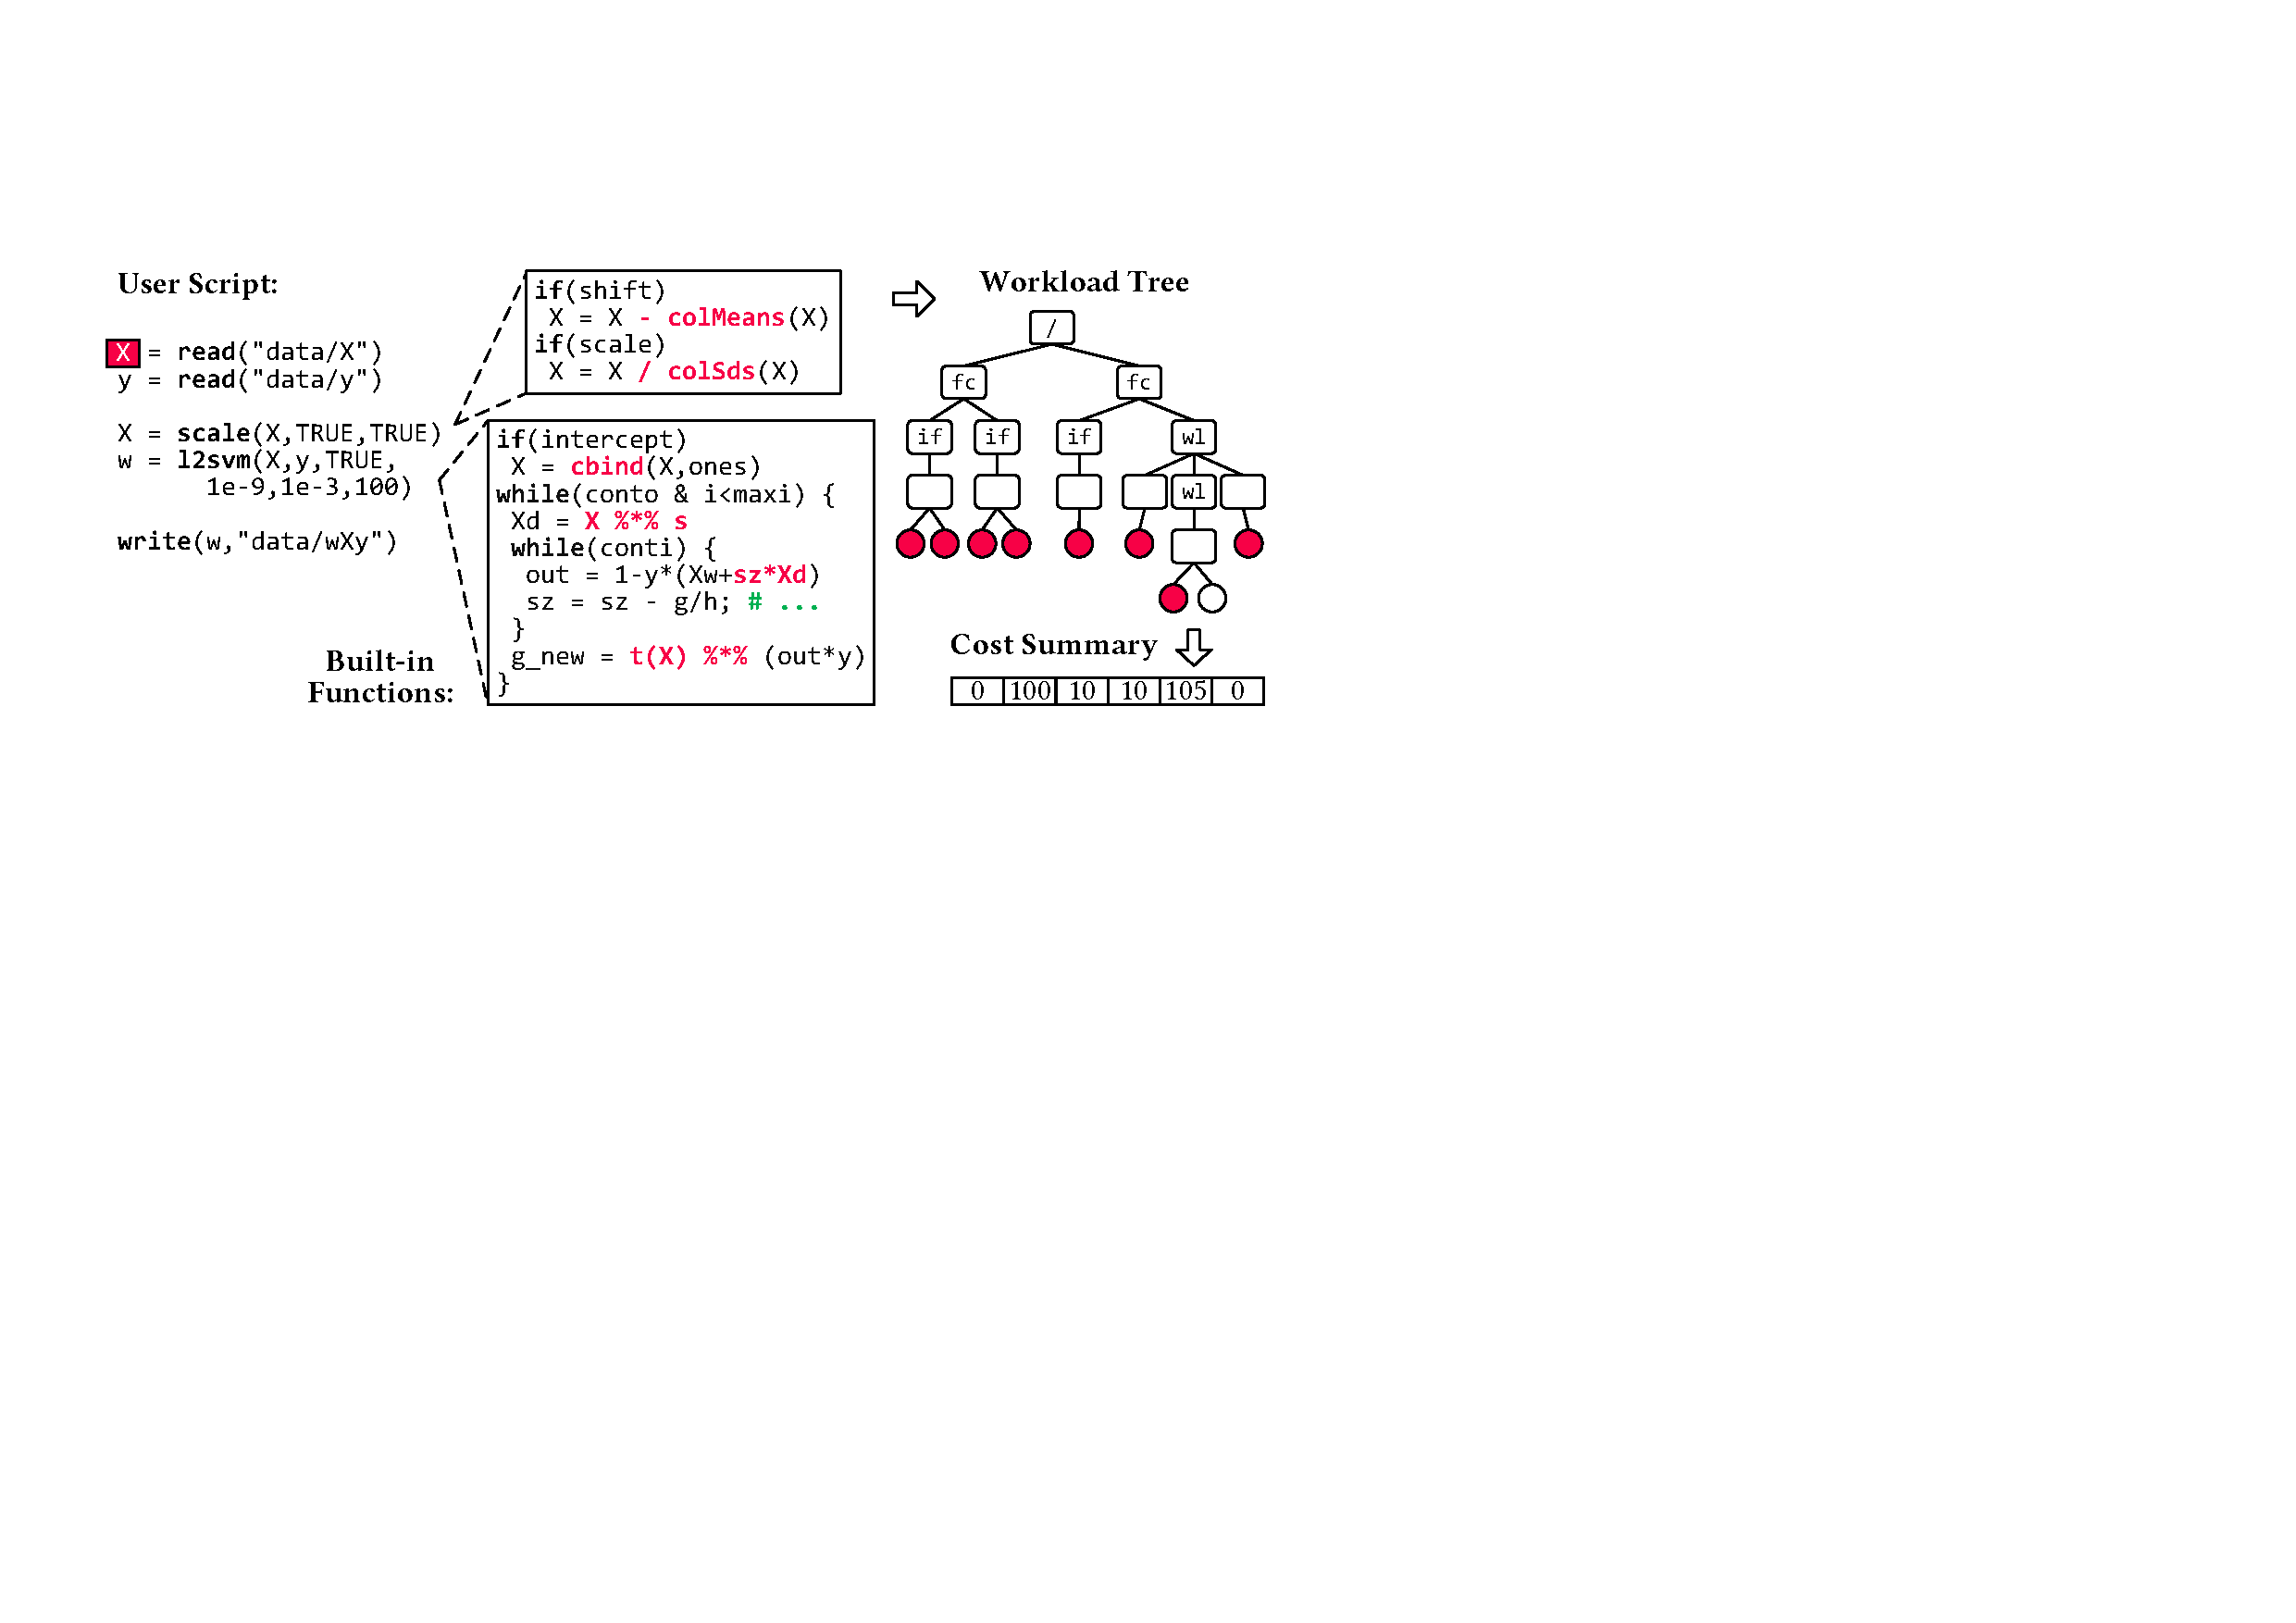
\includegraphics[width=0.8\linewidth]{fig/fig06}
  \vspace{-0.15cm}
  \caption{\label{fig:wtree}
  Example showing a user script that reads a feature matrix \mat{X} and label vector \mat{y},
  normalizes \mat{X} to mean 0 and standard deviation 1, and then trains an l2-regularized support vector machine.
  These functions are themselves linear-algebra scripts.
  Assuming \mat{X} as a compression candidate, we extract the workload tree at the right,
  which contains 2 function calls, 3 if branches,
  2 nested while loops and 8 compressed operations and 1 decompression.
  Aggregating the workload tree yields a cost summary for categories of operations.
  }
  % Workload Tree Extraction.
  \Description{}
\end{figure}

% \begin{example}[Example Workload Tree]
%   \label{ex:wtree} Figure~\ref{fig:wtree} shows an example user script that reads a feature matrix \mat{X} and label vector \mat{y},
%   normalizes \mat{X} to mean 0 and standard deviation 1, and then trains an l2-regularized support vector machine.
%   These functions are themselves linear-algebra scripts.
%   Assuming \mat{X} as a compression candidate, we extract the workload tree at the right,
%   which contains two function calls, three if branches,
%   two while loops and eight compressed operations and one decompression.
%   Aggregating this workload tree yields a cost summary (for categories of operations).
% \end{example}

\textbf{Workload Tree Extraction:}
Our initial candidate selection and optimization approach relies on heuristics.
We make a linear scan over the program, and extract compression candidates by operation type (e.g., persistent reads, comparisons, \texttt{ctable}, and rounding) as well as shape constraints (dimensions, and row/column ratios).
Together, these heuristics find good candidates while keeping the number of candidates low.
For each candidate, we then make a scan over the program and extract its workload tree by computing the transitive closure of derived compressed intermediates (based on operation types that are known to produce compressed outputs).
Again in a heuristic manner, we then evaluate individual candidates independently without considering joint effects of groups of compressed intermediates.
This extraction also descents into functions, but via stack-based identification includes only the first level of recursive function calls.
In this context, we prune the unnecessary extraction of workload trees for overlapping intermediates.
We perform this extraction at the end of inter-procedural analysis (IPA).
At this point, literals and size information have been propagated across the program and into amenable functions, and many simplifications have been performed.
In Figure~\ref{fig:wtree}, we would have propagated the shift, scale, and intercept flags, removed unnecessary branches, and inlined the scale function into the main program.

\textbf{Cost Evaluation:}
The cost summaries computed from the workload tree serve two purposes: for comparing uncompressed operations,
and for guiding compression planning.
We compute both frequencies and costs, where the latter utilizes the cost functions from Table~\ref{tab:cost}.
% The frequencies ignore size differences, but because many intermediates reflect the candidate shape---while row or column aggregations decompress---they represent the workload mix reasonably well.
We organize the cost summaries by categories of operations with different behavior in compressed space: (0) Decompression, (1) Overlapping Decompression, (2) LMM, (3) RMM, (4) TSMM, (5) Dictionary-Ops, and (6) Indexing-Ops.
Decompression is the frequency of regular decompressions,
while overlapping decompression converts the overlapping output into uncompressed form if operations
are not applicable on partial aggregates; both counts are multiplied by number of columns in each occurrence.
LMM is multiplied by the number of rows on the left, RMM multiplied by the number of columns on the right, and TSMM includes counts of compressed multiplications and transpose-self multiplications and is multiplied by the number of columns.
Dictionary operations can be performed directly on the compressed dictionaries (e.g., sum or element-wise scalar operations).
Finally, Indexing refers to slicing of batches or blocking during broadcasting.
If the cost evaluation suggests that compressing an intermediate may be beneficial, we make the cost summary globally available, and inject the related \texttt{compress} directive.
% \textbf{Compress/Decompress Directives:}
%  and place additional \texttt{decompress} directives if needed to handle cases that are difficult to decide at runtime.
% For example, Figure~\ref{fig:wtree} shows an RMM yielding a compressed intermediate \texttt{Xd} in overlapping state.
% This intermediate is used in the inner loop by an element-wise scalar multiplication but subsequently decompressed into non-overlapping state.
% In order to avoid decompression per iteration, we can place a \texttt{decompress} before the inner loop.

\textbf{Compression Planning:}
The \texttt{compress} directives injected into the execution plan, perform compression as described in Section~\ref{sec:compressalg}, but for workload-awareness get a cost summary. The workload mix influence the selection of column group types, co-coding decisions, and tuning for compression ratios.
During classification and co-coding, we estimate the column costs from the sample, and then use these costs to decide on column groupings instead of grouping purely for compression ratios.
However, including I/O costs also enables adapting the compression plans for large out-of-core datasets where good compression ratios are important to fit data in memory and/or reduce I/O. Local compression directly leverages the cost summaries, while for distributed compression, we serialize the cost summaries and compress blocks independently.

\textbf{Adaptive Compression:} In our federated learning backend \cite{Baunsgaard0CDGG21,Baunsgaard0IKLO22}, 
standing worker processes execute continuously incoming
operation requests from multiple tenants. \name\ also supports these
dynamically changing workloads by summarizing cost vectors of previously
executed operations and triggering asynchronous compression to adapt the
compressed representation when needed.


\subsection{Workload-aware Execution Planning}
\label{sec:wlc2}

In the context of hybrid runtime plans---composed of local in-memory, and distributed Spark operations---after compression, opportunities for compiling more efficient plans arise.
Specifically, we can compile operations on compressed intermediates to local operations, where uncompressed operations would exceed the memory budget and fallback to distributed runtime plans.

\textbf{Program Restructuring:} The challenge is that compression happens at runtime, and thus, the estimated and actual compressed size is unknown during initial compilation. Accordingly, we create---similar to data-dependent operators with unknown output shapes \cite{BoehmBERRSTT14}---artificial recompilation opportunities by splitting basic blocks after injected \texttt{compress} directives. If a block contains multiple, independent \texttt{compress} operators, we create a single cut for all.

\textbf{Compression-aware Recompilation:}
If an operator is marked for distributed operations due to unknown input/output dimensions or sparsity during initial compilation,
the entire DAG (basic block) is marked for recompilation during runtime.
Workload-aware compression leverages this infrastructure for obtaining the actual size of compressed in-memory matrices,
and propagating the compressed size bottom-up through the DAG.
With this updated size information, we can compile and execute refined partial execution plans.
Affected decisions include selected execution types (local vs Spark), and physical operators including broadcasting.
